\chapter{Gittergenerierung}

\section{blockMesh}
\textit{blockMesh} ist ein einfacher Gittergenerator für blockstrukturierte (Hexaeder) Gitter. \textit{blockMesh} benötigt als input die datei \textit{constant/polyMesh/blockMeshDict} in welcher die Geometrie und Gittergenerierung festgelegt werden. \autoref{fig:blockmesh} zeigt ein solches Gitter.
\\
Aufgerufen wird \textit{blockMesh} normalerweise ohne Parameter im Wurzelordner der Simulation.

\begin{figure}[htb]
  \centering
  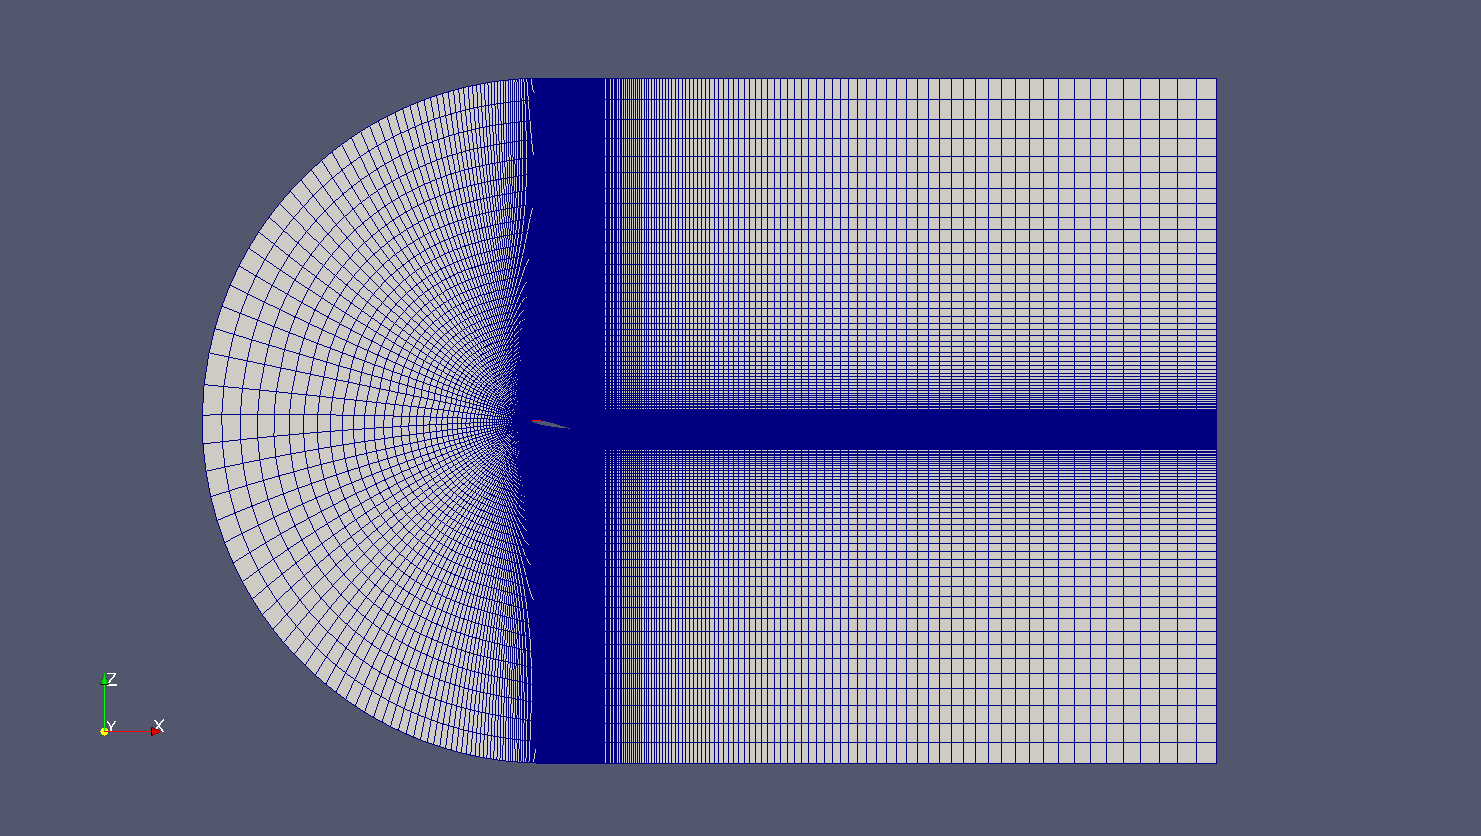
\includegraphics[width=0.95\linewidth]{Abbildungen/blockmesh} 
  \caption[blockMesh Gitter]{Ein mit \textit{blockMesh} generiertes Gitter eines NACA 0012 Flügelprofils. Deutlich zu erkennen ist das Grading im Gitter.}
  \label{fig:blockmesh}
\end{figure}

\autoref{lst:blockMeshDict} zeigt das zur Generierung des in \autoref{fig:blockmesh} genutzte \textit{blockMeshDict}.


Grundsätzlich ist die Gittergenerierung relativ einfach, einige Punkte sind jedoch zu beachten: 
\begin{itemize}
  \item scaleToMeters: Der Parameter \textit{scaleToMeters} (Zeile 18 in \autoref{lst:blockMeshDict}) \textit{blockMeshDicts} ermöglicht es die zu erstellenden Gitter automatisch zu skalieren. Dieser Parameter kann schnell zu Fehlern in den Rechnungen führen, da die Größe des Gitters nicht sofort erkennbar ist und dadurch die zu simulierenden Größen, welche von der Gitterlänge (bspw. Geschwindigkeit, kinematische Viskosität) schnell um Größenordnungen abweichen können. 
  \item boundary: Die Randbedingungen der Gitter werden bereits im \textit{blockMeshDict} festgelegt (in \autoref{lst:blockMeshDict} ab Zeile 116). Dabei ist wichtig, dass die richtig Option gewählt wird. Es stehen in OpenFOAM verschiedene Randbedingungen zur Verfügung (Siehe dazu Kapitel OpenFOAM). Ist noch nicht sicher, um welche Art Randbedingung es sich handelt, ist \textit{type patch} die beste Wahl. 
  \item Uhrzeigersinn: Sollte es beim Generieren des Gitters zu Schwierigkeiten kommen, so lohnt es sich immer die Reihenfolge der abgezählten Knoten (\textit{vertices}) zu überprüfen. Sind diese nicht in der richtigen Reihenfolge kommt es zu Verdrehungen innerhalb des Gitters.
\end{itemize}

\newpage

\section{snappyHexMesh}

\textit{snappyHexMesh} generiert aus einem blockstrukturierten Gitter (blockMesh) ein hybrides Gitter. Mit diesem Tool können bequem komplexe Geometrien in Gitter umgesetzt werden. \autoref{fig:snappy_geometry} zeigt den schematischen Aufbau. Dabei wird von der komplexen Geometrie ein Oberflächengitter (In \autoref{fig:snappy_geometry} als STL surface bezeichnet) benötigt, welches von dem blockstrukturietem Gitter umgeben ist. Das Tool unterstützt viele Oberflächengitter (u.a.: STLs). Als zusätzliche Fähigkeit können prismatische Oberflächenzelle generiert werden, welche (Druck)Gradienten besser abbilden können. Das Tool ist voll parallelisiert, diese Möglichkeit sollte auch genutzt werden, da der Speicherverbrauch hoch ist (pro 1Mio Zellen etwa 1 GB RAM)
\\
Der Aufruf von \textit{snappyHexMesh} erfolgt aus dem Wurzelordner der Simulation. Als nützliche Parameter seinen hier die folgenden aufgezählt:
\begin{itemize}
	\item \texttt{-parallel} soll \textit{snappyHexMesh} parallel genutzt werden, so ist dieser Parameter unerlässlich.
	\item \texttt{-overwrite} \textit{snappyHexMesh} schreibt alle drei Bearbeitungschritte in eigene Zeitordner; ist dies nicht gewünscht (da meist unpraktikabel), hilft dieser Parameter. Das Gitter wird in den \texttt{constant} Ordner geschrieben.
\end{itemize}
\begin{figure}
\centering
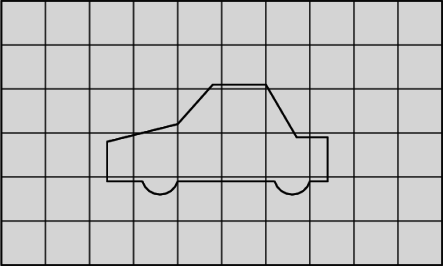
\includegraphics[width=0.7\linewidth]{Abbildungen/snappy_geometry2}
\caption[Geometriedefinition snappyHexMesh]{Geometrie innerhalb eines blockstrukturierten Gitters für die Gittergeneration mit snappyHexMesh. Das blockstrukturierte Gitter muss die Oberfläche überall dort umschließen, wo es zu einer Interaktion zwischen Fluid und Geometrie kommen soll.}
\label{fig:snappy_geometry}
\end{figure}


\textit{snappyHexMesh} wird durch eine Inputdatei (\textit{system/snappyHexMeshDict}) gesteuert. Die Gittergenerierung mit \textit{snappyHexMesh} lässt sich in drei Schritte unterteilen.
\begin{itemize}
	\item Verfeinern	(\textit{castellatedMesh})
	\item Glätten		(\textit{snap})
	\item Oberflächenzellen hinzufügen	(\textit{addLayers})
\end{itemize}
Das \textit{snappyHexMeshDict} ist diesen Schritten entsprechend gegliedert. Zunächst wird die Geomtrie festgelegt (\autoref{lst:snappyHexMeshDictGeometry}):

\begin{dict}{Geometriedefinition innerhalb von \textit{snappyHexMeshDict}}{lst:snappyHexMeshDictGeometry}[ht]
geometry
{
    oberflaeche.stl
    {
        type triSurfaceMesh;
        name oberflaeche;
    }

    verfeinerung
    {
        type searchableBox;
        min (-1.0 -0.7 0.0);
        max ( 8.0  0.7 2.5);
    }
};
\end{dict}

Dabei sind in \textit{snappyHexMesh} mehrere Typen von Geometrien erlaubt:
\begin{itemize}

	\item \texttt{closedTriSurfaceMesh}: benötigt als Input eine \underline{geschlossene} Oberflächengeometrie
	\item \texttt{distributedTriSurfaceMesh}: \todo{raus finden was das ist}
	\item \texttt{searchableBox}: generiert eine Box über die längste Diagonale fest. Inputparameter sind \textit{min(x y z)} und \textit{max(x y z)}.
	\item \texttt{searchableCylinder}: generiert einen Zylinder. Inputparameter sind \textit{min (x y z)}, \textit{max(x y z)} und \textit{radius r}.
	\item \texttt{searchableDisk} \todo{testen}
	\item \texttt{searchablePlane} \todo{testen}
	\item \texttt{searchablePlate} \todo{testen}
	\item \texttt{searchableSphere}: generiert eine Kugel. Inputparameter sind \textit{radius r} und \textit{centre (x y z)}
	\item \texttt{searchableSurfaceCollection} \todo{dafuq?}
	\item \texttt{searchableSurfaceWithGaps} \todo{dafuq?}
	\item \texttt{triSurfaceMesh}: benötigt als Input eine Oberflächengeometrie. 
	
\end{itemize}

Danach folgen die Einstellung für das Verfeinern der Zellen, dem ersten Schritt innerhalb von \textit{snappyHexMesh} (\textit{castellatedMeshControls})

\begin{dict}{\textit{castellatedMeshControls} innerhalb von \textit{snappyHexMeshDict}}{lst:snappyHexMeshDictCastellated}
castellatedMeshControls
{
	// maximal zulässige Anzahl von Zellen pro Prozessor
	// ACHTUNG: bricht Verfeinerung ab sobald Anzahl erreicht ist
    maxLocalCells 100000;

	// maximal zulässige Anzahl von Zellen über alle Prozessoren summiert
    // ACHTUNG: bricht Verfeinerung ab sobald Anzahl erreicht ist
    maxGlobalCells 2000000;

	// sollten weniger als diese Anzahl an Zellen verfeinert werden, wird abgebrochen
    minRefinementCells 10;

	// maximal zulässiges Ungleichgewicht an Zellanzahlen zwischen Prozessoren. Wird dieses Niveau überschritten, werden die Zellen neu verteilt
    maxLoadUnbalance 0.10;

	// Anzahl an Zellschichten zwischen den Verfeinerungen
    nCellsBetweenLevels 3;

	// wird das zusätzliche Tool surfaceFeatureExtract genutzt wird die davon generierte Geometrie hier eingebunden und das Verfeinerungslevel festegelegt
    features
    (
        {
            file "motorBike.eMesh";
            level 6;
        }
    );

	// die Oberflächen zu denen hin verfeinert werden soll, werden hier festgelegt. Dabei kann es sich sowohl um die vorher eingelenen Oberflächengeometrien aus dateien als auch um intern festgelegte Geomtrien, bsp searchableSphere handeln.
    refinementSurfaces
    {
        oberflaeche
        {
            level (min max);
        }
    }

	// Dieser Winkel zwischen zwei angrenzenden Zellen entscheidet darüber, ab wann das nächste Verfeinerungslevel an der Oberfläche eingesetzt werden soll. Start bei min.
    resolveFeatureAngle 45;

	// Soll ein ganzer Zellbereich innerhalb eines bestimmten Raumes auf ein bestimmtes Maß verfeinert werden, wird dies hier festgelegt
    refinementRegions
    {
        refinementBox
        {
            mode inside;
            levels ((1E15 4));
        }
    }

	// diese Koordinate entscheidet darüber welcher Teil des Gitters behalten wird; der innerhalb der Geometrie oder der ausserhalb.
    locationInMesh (3.0001 3.0001 0.43);

	\todo{was ist das?}
    allowFreeStandingZoneFaces true;
}\end{dict}

Nach dem dieser Schritt abgeschlossen ist, ist das Gitter sowohl innerhalb als auch ausserhalb der Geometrie zur Geometrie hin verfeinert (siehe \autoref{fig:snappy_refinement}). 

\begin{figure}
\centering
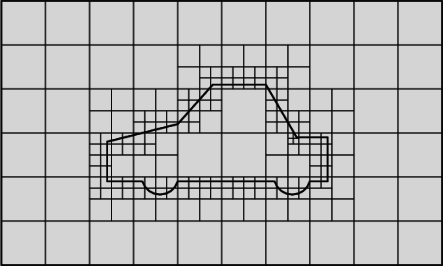
\includegraphics[width=0.7\linewidth]{Abbildungen/snappy_refinement}
\caption[Zellverfeinerung snappyHexMesh]{Die Zellverfeinerungen in der Umgebung der Oberflächengeometrie.}
\label{fig:snappy_refinement}
\end{figure}

Mit Hilfe des Parameters \texttt{locationInMesh (x y z)} wird nun entschieden welcher Teil des Gitter erhalten wird und welcher Teil entfernt wird. Dies gilt ausdrücklich nur wenn es sich bei der Geometrie um eine Wand handelt. Es ist grundsätzlich auch möglich die Verfeinerungen in beide Richtungen beizubehalten. 
\\
Nach dem Ausschneiden sieht das Gitter wie folgt aus (\autoref{fig:snappy_castellated}):

\begin{figure}
\centering
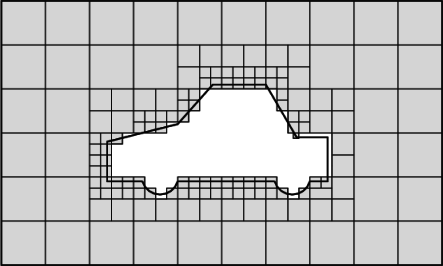
\includegraphics[width=0.7\linewidth]{Abbildungen/snappy_castellated}
\caption[Ungeglättetes, verfeinertes Gitter in snappyHexMesh]{Das ungeglättete, verfeinerte Gitter in snappyHexMesh.}
\label{fig:snappy_castellated}
\end{figure}

Auf die Einstellungen für die Verfeinerungen folgen die Einstellungen für das Glätten der Oberfläche, der zweite Schritt innerhalb von \textit{snappyHexMesh} (\textit{snapControls}, \autoref{lst:snappyHexMeshDictSnap})

\begin{dict}{\textit{snapControls} innerhalb von \textit{snappyHexMeshDict}}{lst:snappyHexMeshDictSnap}
snapControls
{
	// Dieser Parameter legt fest wie viele Iterationen (Wiederholungen) snappyHexMesh darauf verwenden darf die Oberfläche zu glätten.
    nSmoothPatch 3;

	// Dieser Faktor legt die Auflösungtoleranz fest; Die tatsächliche Toleranz entspricht der lokalen Kantenlänge multipliziert mit diesem Faktor. 
    tolerance 2.0;

	// Lösungsiterationen des Gleichungslösers, welcher die Gitterpunkte verschiebt
    nSolveIter 30;

	// Relaxationsiterationen für den Gleichungslöser	
    nRelaxIter 5;

	// Die folgenden Parameter gelten nur für den Fall das mit surfaceFeatureExtract gearbeitet wurde
    nFeatureSnapIter 10;

    implicitFeatureSnap false;

    explicitFeatureSnap true;

    multiRegionFeatureSnap false;
}
\end{dict}

Nach erfolgreicher Beendigung dieses Schrittes hat das Gitter folgende Form (\autoref{fig:snappy_smoothing}):
\begin{figure}
\centering
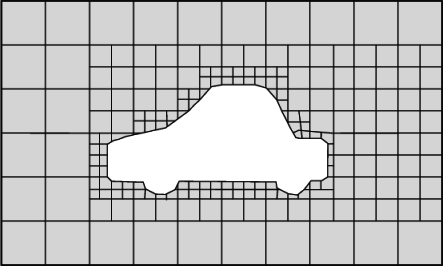
\includegraphics[width=0.7\linewidth]{Abbildungen/snappy_smoothing}
\caption[geglättetes Gitter mit snappyHexMesh]{Das an der Oberfläche geglättete Gitter.}
\label{fig:snappy_smoothing}
\end{figure}

Im letzten Schritt werden die Prismenschichten an den festgelegten Oberflächen generiert. Hierzu werden die folgenden Einstellungen benötigt (\autoref{lst:snappyHexMeshDictAddLayers}):

\begin{dict}{\textit{addLayerControls} innerhalb von \textit{snappyHexMesh}}{lst:snappyHexMeshDictAddLayers}
addLayersControls
{
    // Hier wird angegeben, ob es sich um zum Grundgitter relative Größenangaben (true) oder um absolute Größenangaben (false) handelt. 
    relativeSizes true;

    layers
    {
        geometriename    //nicht name der datei, sondern der name des patches
        {
            nSurfaceLayers 3;
        }
    }

	// relativer Wachstumsfaktor
    expansionRatio 1.0;
	
	// relative Dicke der letzen prismatischen Zellschicht zur unveränderten Grundgitterzelle
    finalLayerThickness 0.3;

	// relative Mindestdicke
    minThickness 0.1;

	// sollten bestimmte Bereich nicht mit Zellen bedeckt werden können, kann die Anzahl der nGrow Iterationen helfen Bedeckung zu erreichen.
    nGrow 0;

	// Ab welchem Winkel zwischen zwei Zellen sollen keine Zellen mehr generiert werden
    featureAngle 60;

	// finger weg \todo{dafuq tis shit?}
    slipFeatureAngle 30;

	// relaxationsiterationen
    nRelaxIter 3;

	// iterartionen zum Glätten der Flächennormalen 
    nSmoothSurfaceNormals 1;

    // Glättungsiterationen des internen Gitters
    nSmoothNormals 3;

   	// iterationen zum glätten der Zellschichtdicken
    nSmoothThickness 10;

    // Ab wann das Glätten der Dicke unterbrochen werden soll; entspricht dem Verhältnis von Zelldicke zu Fläche
    maxFaceThicknessRatio 0.5;

	// keine ahnung
    maxThicknessToMedialRatio 0.3;

	// ebenfalls keine ahnung
    minMedianAxisAngle 90;

    // bis hier her hat eh niemand gelesen
    nBufferCellsNoExtrude 0;

	// Maximale Iteration von Iterationen
    nLayerIter 50;
}
\end{dict}

\begin{figure}
\centering
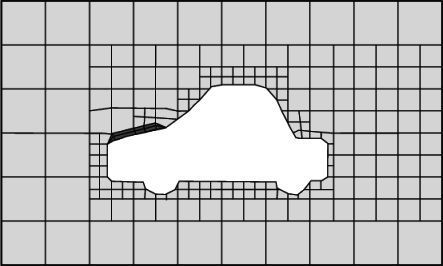
\includegraphics[width=0.7\linewidth]{Abbildungen/snappy_addlayers}
\caption[Prismenschichten snappyHexMesh]{Die Abbildung zeigt das Hinzufügen von prismatischen Zellschichten an der Oberfläche der Geometrie.}
\label{fig:snappy_addlayers}
\end{figure}


\section{proprietäre Gittergeneratoren}

Es existieren eine Reihe freiere und propritärer Gittergeneratoren, für welche OpenFOAM Konvertierungstools zur Verfügung stellt.

\begin{itemize}
	\item[liste:]
\end{itemize}

\newpage